\documentclass[12pt]{article}

%%%%%%%%%%%%%%%%%%%%%%%%%%%%%%%%%%%%%%%%%%%%%%%%%%%%%%%%%%%%%%%%%%%%%%%%%%%%
%%%%%%%%%%%%%%%%%%%%%%%%%%%%%%%%%%%%%%%%%%%%%%%%%%%%%%%%%%%%%%%%%%%%%%%%%%%%
%
% This example requires the a version of advi later than May 7
%
%%%%%%%%%%%%%%%%%%%%%%%%%%%%%%%%%%%%%%%%%%%%%%%%%%%%%%%%%%%%%%%%%%%%%%%%%%%%
%%%%%%%%%%%%%%%%%%%%%%%%%%%%%%%%%%%%%%%%%%%%%%%%%%%%%%%%%%%%%%%%%%%%%%%%%%%%

%%% Some macros
\usepackage {fullpage}
\usepackage {advi-annot}
\usepackage {wedit}
\usepackage {../../doc/manual}

\usepackage {color}
\usepackage {graphicx}
\usepackage {calc}
\usepackage {pst-node}
\usepackage {array}
\usepackage {tabularx}

\def \ActiveDVI {Active-DVI}
\def \WhizzyTeX {{Whizzy\kern -0.3ex\raise 0.2ex\hbox{\let \@\relax\TeX}}}
\def \WhizzyEdit {Whizzy\sc 
\raise 0.2ex \hbox{E}\kern -0.2ex%
\lower 0.0ex \hbox{d}\kern -0.2ex%
\lower 0.2ex \hbox{i}\kern -0.5ex%
\raise 0.2ex \hbox{T}}%

\title{\huge \WhizzyEdit}
\author {Didier R{\'e}my}

\begin{document}

\maketitle

\begin{abstract}
This requires the use of \verb"advi" and of a
recent version that recognized \verb"advi: edit" specials.
See the {\ActiveDVI} and {\WhizzyEdit} related parts of the documentaion.
\end{abstract}

\section{Overview}

{\WhizzyEdit} requires {\ActiveDVI} and {\WhizzyTeX} to work in harmony. 
Actually, {\WhizzyEdit} requires very little {\WhizzyTeX} machinery, which we
describe below. Most of the work resides in the {\ActiveDVI} engine. 
Then, to benefit from {\WhizzyEdit}, one must write style files that
instrument some of the latex commands. 



\section {Tests}

\vspace {8em}

\makeatletter

\makeatletter

\noindent
\psset{boxsep=0pt,framesep=0pt}
\weditcirclenode{x=6.0946,y=4.7659,w=6.5153}
  [boxsep=0pt,framesep=0pt,fillstyle=solid,fillcolor=cyan]{A}%
  {Left \\adjusted\\ circle}%
\weditcirclenode*{x=24.4620,y=7.7952,w=2.4906}
   [boxsep=0pt,framesep=0pt,fillstyle=solid,fillcolor=cyan]%
   {A}{Centered\\ circle}%

%% \newcommand{\weditovalnode}[1]{\@ifnextchar [{\weditovalnode@i{#1}}
%% {\weditovalnode@ii{#1}{}}}
%% \def \weditovalnode@i#1[#2]{\weditovalnode@ii{#1}{#2}}
%% \def \weditovalnode@ii#1#2#3#4%
%%  {\adviedit{comm=\weditovalnode,#1}%
%%   {\hskip -\adviw\ovalnode[#2]{#3}{\hspace{2\adviw}}\hskip -\adviw
%%    \hbox to 0em{\hss \begin{tabular}{c}#4\end{tabular}\hss}%
%%   }}%
\adviedit{x=16.9091,y=-2.9009,w=6.9359}
  {\hsize \adviw\vbox{aa kj lkj lkjkl ljk jjklj klj  
\adviedit{x=7.6260,y=4.1626,w=4.7126}
  {\circlenode{A}{\hspace{\adviw}}}%
aa a aj lkljk lj l lk }}%
%
\adviedit{x=5.8852,y=-3.5785,w=5.6961,h=4.5772,d=4.1668}
  {\hsize \adviw\vtop{aa kj lkj lkjkl ljk jjklj klj  aa a aj lkljk lj l lk
  }}%
%
\adviedit{x=24.8987,Y=-5.8014,w=9.3456,h=2.9880,d=7.1008}
  {\hsize \adviw\vtop{\vskip -\advih\noindent 
  aa ljl j kjlkj ljl jk j kj  hkj lhj ha hjg hjgkgh jk
su yy iaysuy lkj ljl jk jlk jkl jj}}%

%% vspace
\adviedit{d=13.4629}{\vtop{\vspace \advid}}
\noindent
%% hspace
\adviedit{w=21.3128}{\hspace \adviw}AAA

\adviedit{x=22.2576,y=-4.2045,w=10.7179}
 {\ovalnode{A}
   {\parbox{0.69\adviw}{aa aa  a a aaa hkj npkj a aaa hkj kj kj hkj k j}}}

This is some \adviedit{h=-3.1266,w=5.7692,unit=2em}
 {\bubble{anchor}(\advicw,\advich){buble \\bla bla}}
with a bubble

\adviedit[A]{w=6.5340}
          {\setedit{unit=\adviw}%
           \psset{boxsep=0pt,framesep=0pt}%
           \hbox to \adviw
             {\circlenode{A}{\hspace {\adviw}}\hss
              \adviedit[B]{w=0.6660}{\circlenode{B}{\hspace{\adviw}}}}}

\section{Drawings}


$$
\adviedit{x=14.5131,y=0.8895}{\ovalnode{A}{A}}%
\adviedit{x=6.1570,y=-8.1928}{\ovalnode{B}{B}}%
\adviedit{x=-5.6150,y=0.1397}{\ovalnode{C}{C}}%
\adviedit{x=-9.4247,y=-7.4891}{\ovalnode{D}{D}}%
\ncarc{A}{B}\Bput{\ovalnode{ab}{ab}}
\ncarc{B}{C}\Bput{b\adviedit{w=1.9034}{\ovalnode{E}{\hspace{\adviw}E}}c}
\ncarc{B}{D}
\ncarc[linestyle=dotted]{E}{ab}\Aput{!}
$$



\adviedit{w=1.4587,h=1.3152,d=0.3946,unit=4em}
{\ifdim \adviw<\adviunit \else \advisetw{\the\adviunit}\fi
 \ifdim \advih<\adviunit \else \adviseth{\the\adviunit}\fi
 \ifdim \advid<\adviunit \else \advisetd{\the\adviunit}\fi
 \colorbox[rgb]{\advicw,\advich,\advicd}{\hbox{\hsize 4em\vbox to
4em{\noindent Green \vfil \indent \hfill Red\vfil \noindent Blue}}}}

\vfil

A elliptic snow man
$$
\newcommand{\ov}[1][1]{\ovalnode{A}{\vbox{\vspace{#1\advih}}\hspace{#1\adviw}}}
\adviedit{x=-1.7254,y=11.8108,h=3.3564,w=3.2892}{\ov
\adviedit{x=-4.6935,y=1.8635,h=0.6052,w=1.0700}{\ov[0.2]}%
\adviedit{x=-1.3243,y=1.8767,h=0.5062,w=0.8299}{\ov[0.2]}%
}%
\adviedit{x=3.9626,y=7.5836,h=1.2277,w=6.5467}{\ov}%
\adviedit{x=1.4389,y=-4.3766,h=3.1945,w=4.0175}{\ov}%
\adviedit{x=-6.1000,y=-4.5374,h=2.7535,w=4.0984}{\ov
\adviedit{x=-2.5889,y=-0.5650,h=0.6052,W=1}{\ov[0.2]}%
\adviedit{x=-4.8548,y=-0.3222,h=0.6052,W=1}{\ov[0.2]}%
\adviedit{x=-3.7219,y=-0.5649,h=0.6052,W=1}{\ov[0.2]}%
\adviedit{x=-1.9414,y=-0.1603,h=0.6052,W=1}{\ov[0.2]}%
\adviedit{x=-5.9878,y=0.3253,h=0.6052,W=1}{\ov[0.2]}%
}%
\adviedit{x=-11.8928,y=8.1872,h=1.2194,w=7.4739}{\ov}%
\adviedit{x=-2.6759,y=0.0673,h=8.6809,w=4.6210}{\ov}%
$$
\section{Pictures}

\subsection {A Camel caravan}
Want to play? please move and resize the Camel with the mouse.
Be careful, A Camel may hide another one\ldots.

\indent
\epsbygs
\ignorespaces
\def \caml{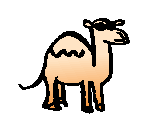
\includegraphics[width=\adviw,height=\advih]{caml.eps}}
%%To adjuste the scale...
\adviedit{x=0.1358,y=0.0110,w=0.4395,unit=\hsize}{%
\vtop to 0.7\adviw {\hbox{%
\setedit{unit=0.2\adviw}%
%%To place and resize each Caml independently, using the same unit.
\adviedit{x=3.8210,y=-1.0322,w=-0.5217,h=0.8348}{\caml}%
\adviedit{x=7.1190,y=-1.3109,w=-1.1080,h=1.0374}{\caml}%
\adviedit{x=1.1410,y=-0.9226,w=1.1661,h}{\caml}%e
\adviedit{x=0.1042,y=-1.4842,w=1.4992,h=1.3165}{\caml}%
\adviedit{x=1.4824,y=-1.4802,w=1.5068,h=1.3165}{\caml}%
\adviedit{x=0.5156,y=-3.1263,w=1.4526,h=1.6604}{\caml}%
\adviedit{x=1.9903,y=-3.1111,w=2.1594,h=1.9219}{\caml}%
}\vfil
}}

\vspace{10em}

Chossing a color:

\medskip
{\setedit{unit=\hsize}%
 \vbox{%
 \hbox{R: \adviedit[R]{w=0.4678}{\xdef\R{\advicw}\hfil}}%
 \hbox{G: \adviedit[G]{w=0.2576}{\xdef\G{\advicw}}}%
 \hbox{B: \adviedit[B]{w=0.5671}{\xdef\B{\advicw}}}%
 \colorbox[rgb]{\R,\G,\B}{\strut \qquad\qquad}
}

\vspace{8em}
\Meaning \whizzy@thelineno

\qquad 
\weditbubble{w=10.5823,h=1.7234}
{\weditbubble{w=3.4823,h=2.3381}
            {\weditbubble{w=-0.4397,h=1.5079}{anchor}{first}}
            {second}}
          {third}

\vspace{5em}

\section{Tabulars, minipages, etc.}

\adviedit{w=7.4988}{%
\begin{minipage}{\adviw}
aaa ahjhk hjk
\end{minipage}}

AAA
$$
\adviedit{w=9.6446}{%
\begin{tabular*}{\adviw}{l@{\extracolsep{\fill}}cr}
aaa &  bbb & ccc\\
\end{tabular*}}
$$

Bellow, the draw dimension is the external width of the tabular
and not the column width...
que l'on re`gle
$$
\adviedit{w=14.6107}{%
\begin{tabular}{lp{\adviw}r}
aaa &  bbb & ccc\\
\end{tabular}}
$$
Unfortunately, the only kown nice fix is to use a command inside...

$$
%Define first line
\newbox \bar 
\setbox\bar =\hbox{\adviedit{w=7.0083}{%
\begin{minipage}[t]{\adviw}
aaa ahjhk hjk
\end{minipage}}}
\edef \foo{\the\wd\bar}
\begin{tabular}{|l|p{\foo}|r|}
\hline
aaa &\unhbox\bar& ccc\\
\hline
aaa &  second line is inlined & ccc\\
\hline
\end{tabular}
$$




\end{document}

% LocalWords:  advi tex moveto whizzy dimen XY
